% 先端芸術音楽創作学会会報テンプレート ver.200908
% By Daichi Ando
% based on ICMC2005

\documentclass{jsarticle}
\renewcommand{\baselinestretch}{0.9}
\usepackage{url}
\usepackage{ascmac}
\usepackage{jssa,amsmath}
\usepackage{mediabb}
\usepackage{listings,jlisting}
\usepackage{graphicx}
\usepackage{plext}
\usepackage{setspace}
\usepackage{color}
\usepackage{setspace}

\definecolor{mygray}{rgb}{0.9,0.9,0.9}

\lstset{%
 backgroundcolor=\color{mygray},
 basicstyle={\small\ttfamily},%
 stringstyle={\small},
 breaklines=true,
 columns=[l]{fullflexible},%
 frame={l},
 numbers=left,%
 tabsize=3,%
 xrightmargin=0zw,%
 xleftmargin=0zw,%
 numberstyle={\scriptsize},%
 stepnumber=1,
 numbersep=1zw,%
 lineskip= -0.5zw%
}

\def\boutenchar{・}
\def\lstlistingname{リスト}

% Title.
% ------
% LaTeX環境によっては,maketitleでエラーが出ることもあるが,強行して良い

\title{Super Collider チュートリアル (3)\\ 
Super Collider Tutorials (3)
}

% Paper Category 論文,報告,連載,書評……など
\category{連載}

% Single address
% To use with only one author or several with the same address
% ---------------
\oneauthor
  {美山 千香士\\Chikashi Miyama} 
  {ケルン音楽舞踏大学\\Hochschule f\"{u}r Musik und Tanz K\"{o}ln} 

\begin{document}

%%% --ページ数等の指定
\makeatletter 
\def\ps@myheadings{% 
\let\ps@jpl@in\ps@plain% 
\def\@evenhead{\reset@font\hfil\leftmark\hfil}% 
\def\@oddhead{\reset@font\hfil\rightmark\hfil}% 
\let\@mkboth\@gobbletwo% 
\let\sectionmark\@gobble% 
\let\subsectionmark\@gobble% 
% 
\def\@oddfoot{\reset@font\hfil-- \thepage --\hfil}% 
\let\@evenfoot\@oddfoot 
} 
\makeatother 

%%% 
%%% 開始ページ数を設定する 
%投稿の段階では無視

\setcounter{page}{ 9 } 
\pagestyle{myheadings} 

%%% 
%%% 論文のVol., No., pp.を設定する 
% 投稿の段階では無視

\markright{\footnotesize \gt 先端芸術音楽創作学会 会報 Vol.1 No.1 pp.9--16 }

%%% 
%%% \maketitleの直後の行に \thispagestyle{myheadings} を挿入する。 

\maketitle
\thispagestyle{myheadings}

%
\begin{abstract}
 本連載では、リアルタイム音響合成環境のSuperCollider(SC)の使い方を、同ソフトを作品創作や研究のために利用しようと考えている音楽家、メディア・アーティストを対象にチュートリアル形式で紹介する。\\
SuperCollider(SC) is a realtime programming environment for audio synthesis. This article introduces SC to musicians and media artists who are planning to utilize the software for their artistic creations and researches.
\end{abstract}
%

\section{今回の目標:MIDIキーボードでSynthを演奏する}
前回は、EnvやEnvGenを使ったエンベロープの作成、SynthDefによるSynthの定義、Routineを用いたメロディーの演奏法等を学習した。今回は、SynthをMIDIキーボードを用いて演奏できるプログラムを作成し、それを通してSCにおけるMIDIメッセージの取り扱いを学習する。

\section{MIDI機器の接続}
\subsection{接続の確認}
SCを立ち上げ、手持ちのMIDIキーボードを繋ぎ、リスト\ref{code:init}のコマンドを実行する。

\begin{lstlisting}[caption=MIDIClientの初期化,label=code:init]
MIDIClient.init;
\end{lstlisting}

MIDIClientはOSのMIDIレイヤーにアクセスするクラスであり、MIDIをSCで扱う際には必ずまず初めにこのクラスに.initメッセージを送る必要がある。

MIDIClient.initを実行すると、MIDIの接続が初期化され、OSから取得した現在のMIDI機器の接続状況がリスト\ref{connection}のように表示される。「MIDI Sources」以下にはコンピュータへのMIDIメッセージの送信元、「MIDI Destinations」以下にはコンピュータからのMIDIメッセージの送信先がMIDIEndPointとして列挙されている。

筆者はAKAIのMIDIキーボードLPK25を接続しているので、このキーボードの名前が表示されている。また、Macを使っているので、IAC Driver\footnote{Inter Application Communication Driver。Macにおけるアプリケーション間でMIDIメッセージを送受信するためのドライバ。これを利用してDAWとSCを連携させることも可能。}もリストされている\footnote{この接続では1つのデバイスに対して、1つのポートであるが、1つのでデバイスで複数のポートが提供される場合もある。}。

\begin{lstlisting}[caption=現在接続されているMIDI機器,label=connection]
MIDI Sources:
  MIDIEndPoint("IAC Driver", "Bus 1")
  MIDIEndPoint("LPK25", "LPK25")
MIDI Destinations:
 MIDIEndPoint("IAC Driver", "Bus 1")
 MIDIEndPoint("LPK25", "LPK25")
\end{lstlisting}

\subsection{入力をテストする}
コンピュータに繋がっている全てのMIDI機器からのメッセージをSCで受け取るためには、MIDIInというクラスに「connectAll」メッセージを送る。その後、MIDIFuncというクラスを用いて様々なMIDIメッセージをSCが受け取った際に、どのようにそれらのメッセージを処理するかを指定する。リスト\ref{code:midi_check}ではMIDIFuncにnoteOnメッセージを送り、MIDIキーボードが打鍵された時にSCに送られてくるMIDIノート・オン・メッセージに対してどのような処理を行うかを定義している。

\begin{lstlisting}[caption=MIDI入力の確認,label=code:midi_check]
MIDIClient.init;
MIDIIn.connectAll;
m = MIDIFunc.noteOn({
  arg vel,note,chan;
  [note,vel,chan].postln
});
\end{lstlisting}

noteOnメッセージの引数として指定された関数内では3つの引数(arg)「vel」、「note」、「chan」が宣言されており、MIDIキーボードを打鍵した際にvelには打鍵の強さ(ベロシティ)、noteには音高を表すMIDIノートナンバー、そしてchanにはMIDIチャンネルが代入される。

このプログラムでは、この3つの要素を1つのArrayに格納し、それに対して.postlnメッセージを送っているので、MIDIキーボードを打鍵すると、[100, 60, 0]のように受信したMIDIノート・オン・メッセージのベロシティ(100)・ノートナンバー(60)・MIDIチャンネル(0)がポスト・ウインドウ表示される。また、ここで定義したMIDIFuncは変数mに格納されている\footnote{MIDIチャンネル・ナンバーは規格上は1から16とされている\cite{midiorg}が、SCではMIDIチャンネルは0から始まる}。

\begin{lstlisting}[caption=関数の解放, label=code:func_free]
m.free;
\end{lstlisting}

プログラムのテストを行った後、リスト\ref{code:func_free}のように必ずMIDIFuncを格納した変数、mに.freeを送り、定義したMIDIFuncの解放を行う必要がある。するとこれ以降、MIDIキーボードを打鍵してもポストウインドウに受け取ったMIDIメッセージが表示されなくなる。

.freeの実行を怠り、さらにもう一度MIDIFunc.noteOnメッセージを実行すると、MIDIノート・オン・メッセージに反応する関数を多重に定義してしまうこととなる。もし、このような意図しない多重定義を行ってしまった場合は、SCの「Language」メニューから「Reboot Interpreter」を選び、一度SCインタプリタをリセットする必要がある。

\section{Synthを演奏する}
\subsection{固定長エンベロープのSynthを演奏する}
\begin{lstlisting}[caption=固定長エンベロープのSynthの例,label=code:jssa]
SynthDef.new("jssa3",{
   arg freq = 440,amp = 0.1;
   a=Saw.ar(freq,amp);
   e=Env.new([0,1,1,0],[0.05,0.1,0.1]);
   Out.ar(0,a*EnvGen.ar(e,doneAction:2));
}).load;
\end{lstlisting}
リスト\ref{code:jssa}は前回作成した"jssa3"というSynthDefである。MIDIキーボードでこのSynthを演奏するにはリスト\ref{code:midi_fixed_length}のようにMIDIFunc.noteOnで登録する関数の中にSynthを組み込む。

\begin{lstlisting}[caption=SynthとMIDIメッセージを関連付ける,label=code:midi_fixed_length]
MIDIClient.init;
MIDIIn.connectAll;
m = MIDIFunc.noteOn({
  arg vel,note,chan;
  Synth("jssa3",["freq",note.midicps,"amp",vel/127]);
});
\end{lstlisting}

これにより、MIDIキーボードの打鍵により、MIDIFuncで登録した関数が実行され、SynthDefで定義したSynthの音が鳴るようになる。このプログラムもテストが終わったら、リスト\ref{code:func_free}を実行し、MIDIFuncを解放する必要がある。

\subsection{MIDIキーボードが手元にない場合}
もし、MIDIキーボードが手元にない場合は、リスト\ref{code:pseudo_midi}の要領でMIDIInクラスに.doNoteOnActionを送り、擬似的に生成したMIDIノート・オン・メッセージをSCに送り、MIDIFuncで登録した関数の反応をテストする事ができる。

\begin{lstlisting}[caption=擬似的にMIDIメッセージを送る,label=code:pseudo_midi]
MIDIIn.doNoteOnAction(0,0,60,64);
\end{lstlisting}

この時の引数は左から、入力ソースID、MIDIチャンネル、MIDIノートナンバー、ベロシティとなる。故に、リスト\ref{code:pseudo_midi}を実行すると、MIDIチャンネル0、MIDIノートナンバー60(C4)、ベロシティ64の擬似MIDIノート・オン・メッセージをSCに送ることができる\footnote{MIDIIn.connectAllを使っているので、入力ソースIDにはどのような値を入れても、反応が得られる}。

\section{音の長さを自在に変える}
前回のチュートリアルでは固定長のエンベロープを用いており、太鼓やチェンバロのように、音の長さを自在に変えるのが不可能であったが、この項では{\bf 可変長エンベロープ}を用いて、ヴァイオリンやオルガンのように、自在に音の長さを変えられるエンベロープを設計する。可変長のエンベロープの設計を行うにはEnvクラスに対して.newではなく、.adsrや.asrなどのメッセージを送る。

\subsection{可変長エンベロープの使用法}

\begin{lstlisting}[caption=可変長エンベロープの定義,label=code:variable_env]
SynthDef("jssa4", {
  arg freq = 440,amp = 0.5,gate = 1;
  e = Env.adsr(0.7,0.5,0.7,1.0);
  a = Saw.ar(freq,amp)*EnvGen.ar(e,gate,doneAction:2);
  Out.ar(0,a);
}).load;
\end{lstlisting}


リスト\ref{code:variable_env}では、Envに.adsrメッセージを送っている。この時メッセージの4つの引数はそれぞれA=アタック・タイム(0.7秒)、D=ディケイ・タイム(0.5秒)、S=サステイン・レベル(アタックの0.7の振幅)、R=リリース・タイム(1.0秒)となる。リストではEnvGenにEnv.adsrで定義したエンベロープを第1引数として渡し、さらに変数gateを第2変数として渡している。このgateの値が0より大きくなった時にEnvGenはエンベロープのアタック部からサステイン部までを出力し、0になった時にリリース部に進める。このように、gateに0を入れるタイミングによって音の長さを自在にコントロールすることができるエンベロープが可変長エンベロープである(図\ref{fig:env})。

\begin{figure}[htbp]
  \begin{center}
    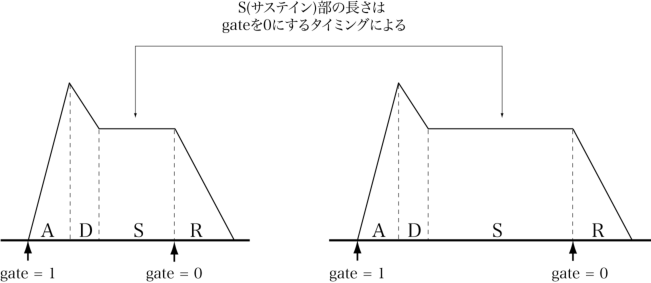
\includegraphics[scale=0.7]{adsr_env.pdf}
  \end{center}
  \caption{可変長エンベロープの例}
  \label{fig:env}
\end{figure}

このSynthDefの定義ではgateの初期値が2行目で「1」に定められているため、このSynthDefを使って発音する際は、引数としてgateに1を指定しなくとも、自動的に発音が始まる。また「doneAction:2」が指定されているため、エンベロープ終了と同時に自動的にこのSynthに使用されたリソースは解放される。

\begin{itembox}[l]{Env}
{\footnotesize 
.adsr({\it attackTime}, {\it decayTime}, {\it sustainLevel}, {\it releaseTime}, {\it peakLevel}, {\it curve}, {\it bias})\\

{\it attackTime}$\cdots${\it gate}を1にしてから{\it peakLevel}到達までの時間。\\
{\it decayTime}$\cdots${\it peakLevel}から{\it sustainLevel}への減衰時間。\\
{\it sustainLevel} $\cdots$サステイン部のレベル。1.0ならば{\it peakLevel}と同じレベルとなる。\\
{\it releaseTime} $\cdots${\it gate}に0が送られてから、完全に消音するまでの減衰に要する時間。\\
{\it peakLevel} $\cdots$エンベロープのピークのレベル。\\
(その他の引数についてはヘルプファイルを参照のこと)
}
\end{itembox}

SynthDefでの定義が終わったら、リスト\ref{code:exec_variable_env}を実行し、可変長エンベロープをテストしてみる。

\begin{lstlisting}[caption=可変長エンベロープのSynthの実行,label=code:exec_variable_env]
x = Synth("jssa4", ["freq", 60.midicps]);
\end{lstlisting}

プログラムを実行すると、C4(ピアノの真ん中のド)が鳴り始めるはずである。これを止めるには、リスト\ref{code:release}のように、.set("gate",0)メッセージをSynthが格納されている変数xに対して送る。すると、エンベロープがリリース部に移行し、1秒後に音が完全に消え、doneActionの効果によりSynthに使われていたリソースが自動的に解放される。
\begin{lstlisting}[caption=可変長エンベロープのリリース,label=code:release]
x.set("gate", 0);
\end{lstlisting}

\subsection{MIDIキーボードと組み合わせる}
このように可変長エンベロープを用いる場合、基本的に発音した全ての音に.set("gate", 0)を送り、音を止める必要がある。これをMIDIキーボードと組み合わせる場合はリスト\ref{code:problem}のように、MIDIFunc.noteOffを用いる。MIDIFunc.noteOffは、MIDIFunc.noteOnがMIDIキーボードが打鍵された時の振る舞いを指定するものであるのに対し、鍵盤から指が離れた時、離鍵した時の振るまいを定義する。

\begin{lstlisting}[caption=可変長エンベロープとMIDIキーボード,label=code:problem]
MIDIClient.init;
MIDIIn.connectAll;
m = MIDIFunc.noteOn({
  arg vel,note,chan;
  x = Synth("jssa4",["freq",note.midicps,"amp",vel/127]);
});
n = MIDIFunc.noteOff({
  arg vel,note,chan;
  x.set("gate",0);
});
\end{lstlisting}

リスト\ref{code:problem}では可変長エンベロープのSynthが使われているので、プログラムを実行して、任意の1つの鍵盤を打鍵すると、MIDIFunc.noteOnで指定した関数が実行され、音がなり始める。そして、その鍵盤の離鍵のタイミングに合わせて、MIDIFunc.noteOffで指定した関数が実行され、x.set("gate",0)を介してエンベロープがリリースされ、音の生成が停止される。

プログラムではMIDIFunc.noteOnとMIDIFunc.noteOffはそれぞれ、変数mとfに格納されている。プログラムのテストが終わったら、mとn両方の変数に.freeを送り、MIDIFuncを解放する(リスト\ref{code:kbd_free})。

\begin{lstlisting}[caption=MIDIFuncの解放,label=code:kbd_free]
m.free;
n.free;
\end{lstlisting}

しかし、このプログラムでは、1つの鍵盤を打鍵し、その鍵盤を離鍵する前に、他の鍵盤を打鍵し、重音や和音の演奏を試みた場合、両方の鍵盤を離鍵しても音が鳴り続けてしまう。図\ref{fig:Synth_problem}は、このプログラムの実行時にF4のキーを押した後に、A4を押し重音を演奏した際に、SC内でどのような処理が行われるかを示したものである。F4のSynthが格納された変数xはA4の打鍵と同時にA4を発音しているSynthに上書きされる。このため、その後、F4のキーを離鍵した時にF4の発音が停止されず、A4の音が停止されてしまい、F4が鳴りっぱなしとなる。

\begin{figure}[htbp]
  \begin{center} 
    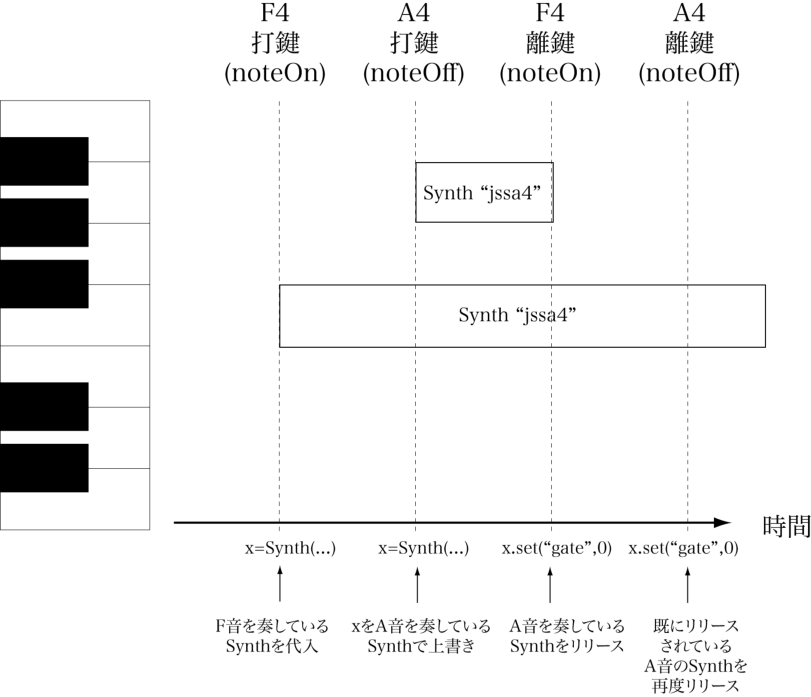
\includegraphics[scale=0.55]{poly_problem.pdf}
  \end{center} 
  \caption{重音・和音の問題}
  \label{fig:Synth_problem}
\end{figure}

\section{ポリフォニック・シンセサイザの実現}

前項のような問題を回避し、重音・和音の演奏ができる{\bf ポリフォニック・シンセサイザ}を実現するには、リスト\ref{code:problem}のx変数のように、一時的にSynthを代入しておくための変数を鍵盤の数だけ用意すればよい。このように多くの変数が必要となる場合は、前回勉強したArrayを使うと効率的である。リスト\ref{code:polyphonic}では、Arrayに.newClearメッセージを送り、中身が「空」(=nil)の127個の要素からなら配列「a」を定義している。これであらゆる鍵盤が打鍵された時に、その鍵盤のMIDIノートナンバーに匹敵する配列のインデックスにSynthを一時的に格納する事ができ、発音とリリースの処理を個別に各音に対して行う事ができるようになる(図\ref{fig:array})。

\begin{figure}[htbp]
  \begin{center}
    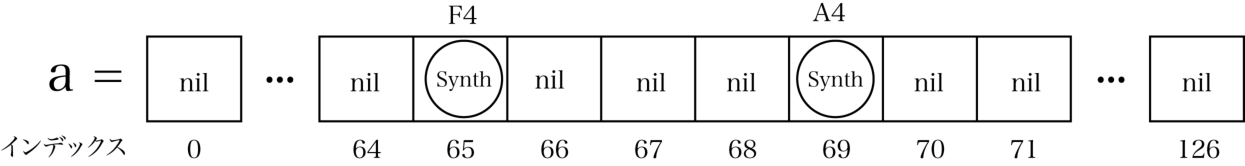
\includegraphics[scale = 0.38]{array.pdf}
  \end{center}
  \caption{配列とSynth}
  \label{fig:array}
\end{figure}

\begin{lstlisting}[caption=ポリフォニック・シンセサイザ,label=code:polyphonic]
MIDIClient.init;
MIDIIn.connectAll;
a = Array.newClear(127);
m = MIDIFunc.noteOn({
  arg vel,note,chan;
  a[note] = Synth("jssa4",["freq",note.midicps, "amp", vel/127]);
});
n = MIDIFunc.noteOff({
  arg vel,note,chan;
  a[note].free;
});
\end{lstlisting}

このプログラムもテストが終わった後にリスト\ref{code:kbd_free}を実行し、MIDIFuncを解放する必要がある。

\section{まとめ}
今回はSCとMIDIの連携、ポリフォニック・シンセサイザのプログラムを学習した。SCではガーベッジコレクションや、エンベロープ関連のクラス、MIDIFuncによるMIDIメッセージの取り回しの良さなどが相俟って比較的簡単にリソース消費の少ない実用的なシンセサイザをプログラムする事ができる。次回はこのシンセサイザに更に様々な機能を追加し、より表現力の高いものにしてゆく。

\bibliographystyle{jplain}
\begin{thebibliography}{citations}
  \bibitem{scsite} {\it SuperCollider}, \url{http://supercollider.sourceforge.net}(アクセス日 2014年1月8日)
  \bibitem{midiorg} {\it MIDI Manufactures Association}, \url{http://www.midi.org}(アクセス日 2014年1月8日)

\end{thebibliography}

\section{著者プロフィール}
\subsection*{美山 千香士 (Chikashi Miyama)}
作曲家、電子楽器創作家、映像作家、パフォーマー。国立音楽大学音楽デザイン学科より学士・修士を、スイス・バーゼル音楽アカデミーよりナッハ・ディプロムを、アメリカ・ニューヨーク州立バッファロー大学から博士号を取得。Prix Destellos特別賞、ASCAP/SEAMUS委嘱コンクール2位、ニューヨーク州立大学学府総長賞、国際コンピュータ音楽協会賞を受賞。2004年より作品と論文が国際コンピュータ音楽会議に12回入選、現在までに世界18カ国で作品発表を行っている。 2011年、DAAD(ドイツ学術交流会)から研究奨学金を授与され、ドイツ・カールスルーエのZKMで客員芸術家として創作活動に従事。近著に「Pure Data-チュートリアル&リファレンス」(Works Corporation 社)がある。現在ドイツ・ケルン音楽大学講師、チューリッヒ芸術大学非常勤講師。ケルン・メディア芸術大学フェロー。チューリッヒICSTのSpatDIFプロジェクト及びMGMプロジェクトにプログラマとして参加している。
\end{document}
